\subsection{Zadania komputerowego przetwarzania biosygnałów na wybranym przykładzie (np. EKG, EMG)}

Sygnały biomedyczne to sygnały, których \textbf{źródłem jest człowiek} – „obiekt” o cechach zmiennych w czasie, podlegających wpływowi osobniczemu. Obiekt jest istotą żywą, do której stosujemy metody inżynierskie w celu obiektywnej oceny jego stanu.


\subsubsection{Klasyfikacja biosygnałów}

Zależnie od źródła pochodzenia, wyróżnić można kilka rodzajów sygnałów biomedycznych:

\begin{itemize}
	\item \textbf{Mechaniczne} - Np. ciśnienie krwi, ruchy wykonywane przez organy lub części ciała, sygnały dźwiękowe (przykładowo szmery w układzie oddechowym),
	\item \textbf{Chemiczne} - Np. współczynnik PH płynów ustrojowych, zawartość określonej substancji składowej,
	\item \textbf{Termiczne} - Np. ciepło emitowane przez poszczególne części ciała,
	\item \textbf{Elektryczne} - Np. EKG, EMG (pochodzące z serca), EEG (pochodzące z układu nerwowego),
	\item \textbf{Magnetyczne} - Powiązane z sygnałami elektrycznymi, ale rzadko wykorzystywane ze względu na trudność ich rejestracji i identyfikacji. \\
\end{itemize}

Ze względu na okresowość można wyróżnić sygnały:
\begin{itemize}
	\item \textbf{Okresowe} - taka sama sekwencja powtarza się co pewien okres czasu.
	\item \textbf{Quasi-okresowe} - bardzo podobna sekwencja powtarza się co pewien okres czasu, bądź poszczególne nieco różnią się czasem trwania. Do takich sygnałów można zaliczyć np sygnały elektryczne emitowane przez serce.
	\item \textbf{Nieokresowe} - nie można wyróżnić powtarzających się sekwencji.
\\
\end{itemize}

Zależnie od stochastyki, podzielić je można natomiast na dwie podgrupy:

\begin{itemize}
	\item \textbf{Stacjonarne} - Statystyczne parametry tych sygnałów nie ulegają zmianie. Przykładowo: norma zawartości żelaza we krwi określana jest odgórnie zależnie od wymiarów organizmu, więc wartość oczekiwana tego parametru nie ulega zmianie w czasie,
	\item \textbf{Niestacjonarne} - Statystyczne parametry tych sygnałów mogą ulec zmianie w czasie. Przykładowo: wariancja wyznaczana na sygnale EKG lub EEG.
\end{itemize}

\subsubsection{Przetwarzanie biosygnałów}

Do najpopularniejszych metody wykorzystywanych w procesie przetwarzania takich sygnałów należą:

\begin{itemize}
	\item \textbf{Filtracja} – Usuwanie lub redukcja pewnych elementów sygnału,
	\item \textbf{Analiza} – Ekstrakcja poszukiwanych cech z sygnału, zazwyczaj poprzez jego segmentację lub parametryzację, pozwalając na konwersję sygnału do postaci wektora cech, który poddany zostać może dalszej analizie,
	\item \textbf{Interpretacja} - Porównanie otrzymanego pomiaru z oczekiwanym wzorcem, wyszukiwanie w nim anomalii lub charakterystycznych elementów.
\end{itemize}

\subsubsection{Analiza sygnału EKG(\textit{elektrokardiogram})}

Sygnał EKG jest napięciem elektrycznym rejestrowanym na ciele poprzez odpowiednio połączone elektrody. Pozwala on zdiagnozować liczne problemy powodowane przez choroby serca, lub zaburzenia jego pracy. Jest on jednym z najczęściej wykorzystywanych i najlepiej zbadanych sygnałów wykorzystywanych w diagnostyce medycznej. \\

Analiza tego sygnału przeprowadzana jest w trzech etapach:

\begin{itemize}
	\item \textbf{Filtracja} - Usuwa określone pasma z pomiaru:
	\begin{itemize}
		\item \textbf{Filtr górnoprzepustowy} - Usuwania dryft linii izoelektrycznej (0.2Hz – 0.5Hz),
		\item \textbf{Filtr szczelinowy} - Usuwa zakłócenia sieci elektroenergetycznej (50Hz),
		\item \textbf{Filtry dolnoprzepustowe} - Usuwają zakłócenia pochodzące z drżeń mięśniowych, aparatury elektromedycznej, oraz artefakty pomiaru (25Hz, 35Hz).
	\end{itemize}
	\item \textbf{Analiza} - Wyznacza charakterysytyczne punkty sygnału (początek i koniec P, QRS, koniec T, lokalizacja Q, R, S, J, amplitudy P, Q, R, S, T, nachylenie S-T) oraz parametry zespołu uśrednionego (uśrednione wartości tych samych charakterystyk dla kilku różnych sygnałów EKG),
	\item \textbf{Interpretacja} - Porównanie cech otrzymanego sygnału (np. odstęp PQ, czas trwania zespołu QRS, amplituda załamka Q, nachylenie odcinka ST) z kryteriami medycznymi dla rożnych zaburzeń (np. blok przedsionkowo-komorowy, rytm nadkomorowy, przerost lewej komory, itp.).
\end{itemize}

\begin{figure}[H]
	\centering
	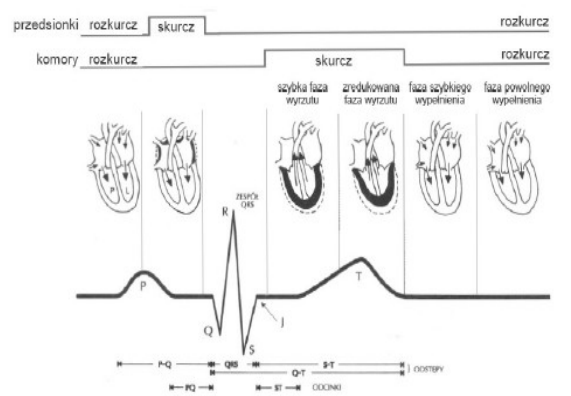
\includegraphics[width=0.7\linewidth]{K4.png}
	\caption{EKG}
\end{figure}

\subsubsection{Analiza sygnału EMG(\textit{elektromiogram})}

Diagnostyka \textbf{czynności elektrycznej mięśni} i nerwów obwodowych za pomocą urządzenia wzmacniającego potencjały bioelektryczne mięśni i nerwów – elektromiografu.
Analiza takiego sygnału z przedramienia pozwala skonstruować \textbf{protezę ręki}. \\

Analiza tego sygnału przeprowadzana jest w trzech etapach:

\begin{itemize}
	\item \textbf{Filtracja} - wchodzący sygnał EMG jest poddawany filtracji (bądź wyostrzaniu/wzmacnianiu).
	\item \textbf{Analiza} – po wyostrzeniu sygnału wykonywana jest parametryzacja, czyli analiza sygnału w wyniku której otrzymuje się zbiór wartości parametrów niosących informację.
	\item \textbf{Interpretacja} - zbiór parametrów tworzy wektor (lub macierz) cech, na podstawie którego dokonuje się klasyfikacji. W bloku klasyfikacji następuje porównanie uzyskanych cech ze znajdującymi się w pamięci wzorcami, które stanowią uogólniony (uśredniony) opis klas.
\end{itemize}

\begin{figure}[H]
	\centering
	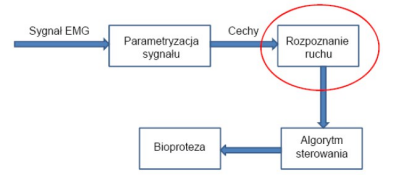
\includegraphics[width=0.6\linewidth]{K4_1.png}
	\caption{EMG - bioproteza}
\end{figure}
